%!TEX encoding = UTF-8 Unicode
%!TEX root = ../Main/thesis.tex
% !TEX spellcheck = en-US
%%=========================================
\documentclass[../Main/thesis.tex]{subfiles}
\begin{document}
\chapter{Introduction}
\label{ch:introduction}

%The organizations Uni Research Health, Centre for the Science of Learning \& Technology (SLATE), Western Norway University of Applied Sciences (HVL), ENOVATE AS and Øygarden Brann og Redning (Øygarden fire and rescue) are currently cooperating on the project ``Inquire Competence for Better Practice and Assessment'' (iComPAss).
%This project does, among other things, study how one could use data driven decision-making to improve the training of firefighters.
%As a part of that study they want to research how and if Bluetooth or similar technologies could be used to track the movements of firefighters when they exercise smoke diving.

Today we have accurate systems for outdoor localization, positioning, and tracking using the Global Positioning System (GPS). 
GPS is available almost everywhere, and because most smartphones have a GPS-antenna it is easy to use in applications.
Unfortunately, GPS does not work well enough indoors to give precise locations.
There are, however, several emerging technologies for indoor localization and tracking, such as light \citep{xiaohan2010improved}, sound \citep{schweinzer2010ultrasonic}, WIFI  \citep{chang2010robust}, and Bluetooth \citep{Takahashi2016}.
None of these systems are commonly available or in widespread use yet, however.

One use-case where precise indoor tracking might be useful is for supporting firefighter smoke diving training. 
As the training building is filled with smoke the visibility is low or nonexistent, thus it is easy to get disoriented or lose track of where you are and where you have been.
Which is the point of the exercise.
For a firefighter it is crucial to check all rooms or parts of a building when searching through it, therefore, smoke diving is one of the important abilities they train.
Smoke diving is also carried out according to competence-based practice, with standards for movement, communication, equipment use, etc.
Yet, there are few tools that provide the divers with data on their performance.
How can you get better at it and learn from your errors, however, if you think you searched all the rooms in the building, and no one is able to tell you that you missed a bedroom?
Did you carry out the search optimally?
And will visualizations of this improve the instructor - trainee dialogue and feedback.

To meet this need for information about firefighters movement and activity in a smoke filled building a system for tracking them while they train was created using Bluetooth Low Energy (BLE) beacons and smartphones to track the firefighters and visualize the data about their movements. 
This visualization can be used in the debriefing and evaluation process after the training with their instructor.
The instructor can also use the data across the teams to see what they need to train on.

\section{Motivation}
The motivation for doing this masters project is that there is a clear need for a tool that provides smoke divers data-based feedback on their activities.
We also want to explore the capabilities of, and learn about the BLE beacons and see how well they perform in an environment like this, which is almost unexplored when it regards use of Bluetooth technology. 

\section{iComPAss project}
This research is part of the ``Inquire Competence for Better Practice and Assessment'' (iComPAss) project which is a cooperation between the organizations Uni Research Health\footnote{Uni Research merged with several other research institute and changed name to NORCE Norwegian Research Centre AS}, Centre for the Science of Learning \& Technology (SLATE), Western Norway University of Applied Sciences (HVL), ENOVATE AS and Øygarden Brann og Redning\footnote{Changed name from Sotra Brannvern to Øygarden Brann og Redning after a organizational restructure as of January 2018} (Øygarden fire and rescue). \todo{finish this section}
\citep{Netteland2016}

IComPAss presented several poster at the LASI-Nordic conference in Copenhagen, Denmark in August 2019, including a poster for the work presented in this thesis \citep{Wake2018}. 
The conference poster is included in Appendix~\ref{app:lasi-poster}.

\section{Collaboration with co-student}
While this research is conducted together with a co-student, Edvard Pires Bjørgen, what is reported in this thesis is my own individual work.
Together we developed the FireTracker system, which comprises an exercise management tool, an android application, and a back end.
I was responsible for the back end, Edvard the exercise management tool, and we shared the responsibility for the android application \citep{Bjorgen2018}.
An overview of the FireTracker system with its data flow is shown in Figure~\ref{fig:system-overview}.

\begin{figure}[h]
	\centering
	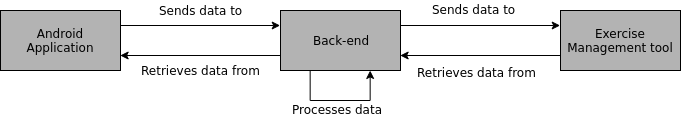
\includegraphics[width=\textwidth]{../fig/system-overview}
	\caption{Overview of FireTracker with data flow}
	\label{fig:system-overview}
\end{figure}

\section{Research Questions}
\label{ch:reserch_questions}
In my master project I will look at how well the Bluetooth Low Energy beacons perform in a smoke diving setting and environment. 
My goal is to answer the following two questions:

\begin{enumerate}
	\item \textbf{How can BLE beacons be used to support firefighter movement tracking under smoke diving training?}
	\item \textbf{Do the beacons provide good enough information for useful feedback?}
\end{enumerate}


\section{Overview of thesis}
This thesis is divided into eight chapters.
The second chapter is an overview of relevant literature and theory.
In the third chapter the research methodology is described.
Chapter four is an overview of the technologies used in the project, and why they where chosen.
The fifth chapter describes the first iteration of the development where requirements are established.
Chapter six is a description of the second iteration of the development, where the first prototype is developed and tested.
In chapter seven the third iteration is described.
Chapter eight is a description of the evaluation of the system.
In chapter nine findings are discussed, and ten eight is the conclusion.


\blankpage

\onlyinsubfile{\bibliographystyle{chicago}}
\onlyinsubfile{\bibliography{../library}}
\end{document}
